\documentclass[12pt]{extarticle}
\linespread{1.8}
\usepackage{fancyhdr,amsfonts,graphicx,wrapfig,sidecap,float,adjustbox,subcaption,indentfirst,amsmath,hyperref}
\usepackage{listings}
\usepackage{color}
\usepackage{gensymb}

\usepackage[right=2.5cm,left=2.5cm,top=2.5cm,bottom=2.5cm]{geometry}

\pagestyle{fancy}
\lhead{Memorial University of Newfoundland}
\rhead{Department of Mathematics and Statistics}
\renewcommand{\headrulewidth}{0.4pt}

\lfoot{Mathematics 2130}
\cfoot{}
\rfoot{Fall 2015, Project 4}
\renewcommand{\footrulewidth}{0.4pt}
\flushbottom
\begin{document}
\begin{titlepage}
\vspace*{2in}
\begin{center}
{\LARGE Road Traffic and Simulations}
\end{center}

\vspace{2cm}

\abstract{This paper aims to provide analysis of traffic. Its flow and density are some of the main focuses. The affects of gradual increasing and decreasing probabilities of deceleration and random stopping is also observed. These are the topics analyzed and discussed in detail. }

\vspace{3in}
\begin{flushright}
\begin{tabular}{l}
Project 4 \\
Mathematics 2130\\
Submitted by: John Hollett\\
Submitted to: Ivan Booth\\
\today
\end{tabular}
\end{flushright}


\end{titlepage}


\lhead{Road Traffic and Simulations}
\rhead{Math 2130}
\lfoot{John Hollett}
\rfoot{\thepage}

%\underheadoverfoot




\section{Introduction}

In this paper, a mathematical model is used to examine the characteristics of traffic flow. This model is a simplified example comparable to real world traffic. For the purposes of this paper, traffic is defined as vehicles interacting on a road. The mathematical model utilizes mechanical processes that remove complexity from real world traffic and simplify it to provide results to be interpreted.

This mathematical model was made with the programming language C$^\#$. The structure and inner mechanics will be discussed later in this paper. In the next section, it is explained what mechanics were used to create the mathematical model used to carry out the analysis.

The goal of this analysis is to provide a better understanding of traffic flow and deadlocking that occurs. Using graphics and the simulation, the performed analysis will provide convincing proof that the actions of drivers can influence reverberating traffic conditions.

\section{Mechanics}

The traffic model used consists of cars and roads. The road described should be considered to be similar to a roundabout. This means the road loops back on itself. Each car is located on a road with other cars where they interact. However, unlike in the real world, these cars cannot cause accidents. The position of these cars is described by:

\begin{align}
\label{e1}
x_{i-1}(t) < x_{i}(t) < x_{i+1}(t)
\end{align}

Where $x$ is the car, $i$ is the index and $t$ is the time in the sequence. This rule is important for maintaining consistent behavior amongst all cars. Without this rule, cars would collide providing inconsistent results. The extent of which cars may move as well as density is described by:

\begin{align}
\label{e2}
v_i(t) &\in \{0,1,2, ..., V_{max}\} \\
\label{e3}
D(C,R) &= \frac{C}{R}
\end{align}

Where $v$ is the velocity of the car at index $i$. The speed of a car is an integer value and the maximum speed is described by $V_{max}$. Density is cars divided by the length of road. Similar to real world traffic, the cars in this model observe the speed limit explicitly. In this model, cars will accelerate when possible and decelerate to avoid accidents. Each car has a probability to deceleration randomly. The rules of acceleration and deceleration are as follows:

\begin{align}
\notag 1)& \ \ v_i(t) < V_{max} : v_i(t+1) = v_i(t) + 1\\ 
\notag 2)& \ \  x_i(t) + v_i(t + 1) \geq x_{x+1}(t) : v_i(t + 1) =x_{i+1}(t) - x_i(t) - 1\\
\label{e4}
3)& \ \ Pr(P < P_{o}) :v_i(t+1) = v_i(t+1) - 1 
\end{align}

The rules above, in the appearing order, are applied to each car in the simulation. After finding the new values, the position of each car is updated. This is done using the formula:

\begin{align}
\label{e5}
 x_i(t + 1) = x_i(t) + v_i(t+1)
\end{align}

Where $x$,$v$ and $t$ is position, velocity and time respectively; $i$ is the car in the list. The rules listed were assembled within a program to create a simulation. The next section will discuss the results of some tests.

\section{Analysis}

This section will cover the different types of tests performed using the simulation. The first set of tests will show the affects of density on cars and the second will examine the probability of random deceleration. This is carried out by adjusting the probability of deceleration and density using equation (\ref{e4}) and (\ref{e3}). The third test will examine the affects of a section of road where the probability of deceleration increases and decreases. The graphs in this report were created by running the simulation for 10000 steps before data is collected.

\subsection{Density Analysis}
\begin{figure}[h!]
	\centering
	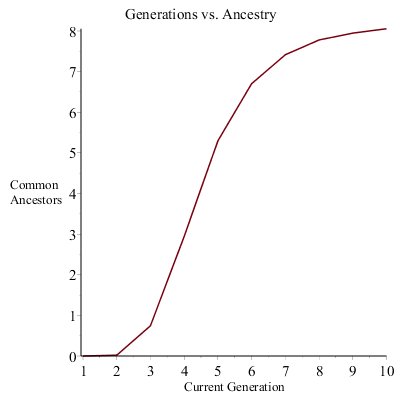
\includegraphics[scale=0.70]{Graph1.png}
	\caption{Cars = 200, Roads = 1000, Prob = 0.05}
	\label{fig:img1}
\end{figure}

In this test, the affect of density is examined. To do this effectively, the length of road and number of cars will be chosen to maximize the data. An arbitrary road length of 1000 was selected. Using equation (\ref{e3}), the observed density is set to 20\%. Deriving the number of cars from the equation, the result is 200. To give the data character, the probability of deceleration will be set to 5\%. The reasoning behind this is explained in the technical details.

Following figure (\ref{fig:img1}), usage of color depicts the results. The colors ordered \{black, red, orange, yellow, green, blue\} are symbolic of the speeds of the cars from 0 to 5. This coloring scheme is constant for all tests in this paper. The data shows streaks of red and black diagonally aligned. This effect is the result of random deceleration on the cars. With the x and y axis describing road segments and time respectively, the colors depict the individual velocities of cars.

The results of the first test performed shown by figure (\ref{fig:img1}) show streaks of red which shows consistent traffic jams over time. As time increases there are small instances of traffic that form and dissipate shown by small spots of red. The difference between these two characteristics is consistent and inconsistent traffic jams. These are caused by small chances in probability where cars decelerate once or twice affecting the pursuing cars. In addition to the chance to decelerate, rules describing velocity make possible instances where cars decelerating to avoid collision may randomly decelerate also.

The next two figures show increasing car density over constant probability of deceleration. These tests were performed with 300 and 400 cars.

\begin{figure}[h!]
	\caption{Roads = 1000, Prob = 0.05}
	\begin{subfigure}{0.50\textwidth}
		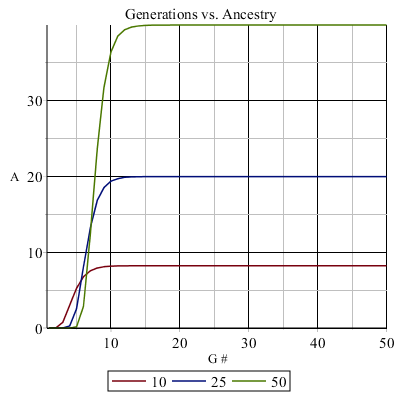
\includegraphics[scale=0.50]{Graph2.png}
		\caption{Cars=300}
		\label{fig:img2}
	\end{subfigure}
	\begin{subfigure}{0.50\textwidth}
		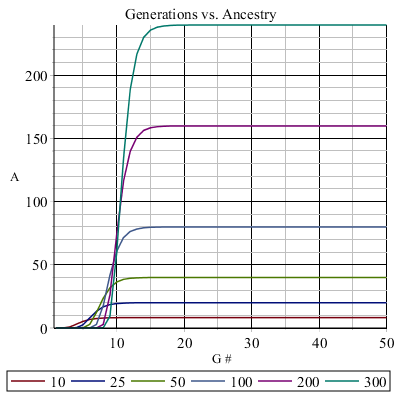
\includegraphics[scale=0.50]{Graph3.png}
		\caption{Cars = 400}
		\label{fig:img3}
	\end{subfigure}
\end{figure}

In figure (\ref{fig:img2}) and (\ref{fig:img3}), observation of red and black streaks is made. This depicts stronger traffic at densities of 30\% and 40\%. Just as the previous figure has shown, there are streaks of consistent and inconsistent traffic. 

The differences between the increasing densities show that traffic is still considerably consistent. Cases where multiple deadlocks merge into larger traffic jam can be observed. This can be explained by referring to the velocity rules. If cars decelerate, that car tries to accelerate to the maximum velocity. 

\subsection{Probability Analysis}
\begin{figure}[h!]
	\centering
	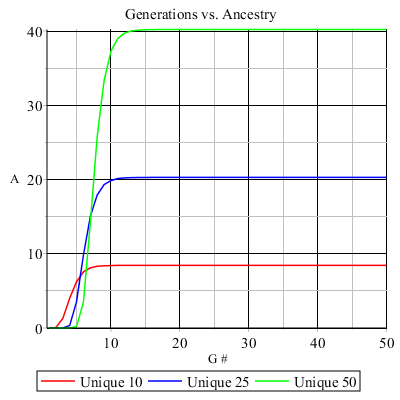
\includegraphics[scale=0.70]{Graph4.png}
	\caption{Cars = 100, Roads = 1000, Prob = 0.05}
	\label{fig:img4}
\end{figure}

In this section, the number of cars remain constant. The density is decided with equation (\ref{e3}). With constant cars, changing probability of deceleration produced different results compared to density.
\begin{figure}[h!]
	\caption{Roads = 1000, Cars = 100}
	\begin{subfigure}{0.50\textwidth}
		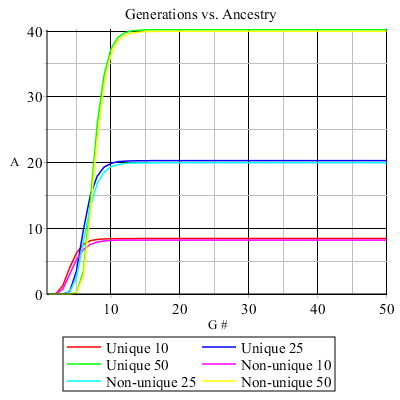
\includegraphics[scale=0.50]{Graph5.png}
		\caption{Probability = 0.25}
		\label{fig:img5}
	\end{subfigure}
	\begin{subfigure}{0.50\textwidth}
		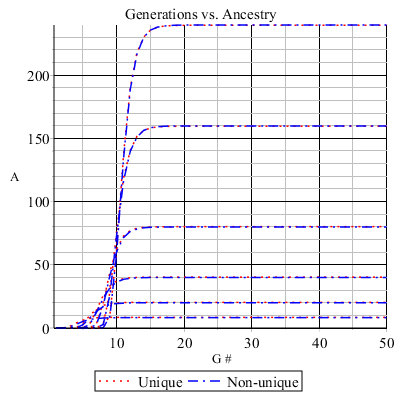
\includegraphics[scale=0.50]{Graph6.png}
		\caption{Probability = 0.40}
		\label{fig:img6}
	\end{subfigure}
\end{figure}
Comparing figure (\ref{fig:img1}) and (\ref{fig:img4}), the difference is 100 cars and 10\% greater chance of deceleration. With less cars under increased probability, the results show the road is traffic free. However, the characteristic observed in figure (\ref{fig:img4}) that is not seen as frequently in the others is white streaks. These streaks represent space between cars. The figure also depicts yellow noise. This is caused by random deceleration as seen in previous figures. This difference is important to note as the decreased density creates better road conditions with low deceleration probability. However, yellow spots indicate road speed not always consistent.

The figures (\ref{fig:img5}) and (\ref{fig:img6}), depict the results of the simulation ran with 25\% and 50\% probabilities of deceleration. In the 25\% sample, more noise is observed and greater consistency of traffic compared to figure (\ref{fig:img4}). The 50\% sample shows a different scenario. This simulation shows proportions of road where deadlock occurs. Smaller instances of traffic dissipating can be observed. Larger instances take longer to dissipate or persist outside the data. The two figures show 25\% probability have faster road velocities compared to the 50\% figure. 

These results show that density affects road velocity more than random deceleration. With 100 cars and 50\% probability of deceleration, lower levels of traffic are observed compared to 200 cars with 5\% probability of deceleration. With these results it can be concluded that density has a greater affect on road conditions than deceleration probability. This is related to the length of road and number of cars present in the system. In a closed circuit, such as the one used in the simulation, it is evident that can traffic extended time to resolve, if ever. In relation to real world, it would be sufficient to state traffic will improve as the leading cars accelerate. 
\begin{wrapfigure}[15]{r}{0.475\textwidth}
	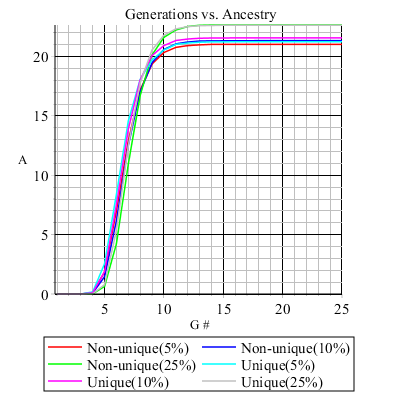
\includegraphics[scale=0.50]{Graph7.png}
	\caption{Cars = 200, Roads = 1000, \newline Probability = $0.10 < P < 0.22$}
	\label{fig:img7}
\end{wrapfigure}
\subsection{Alternate Analysis}
\subsubsection{Normal Distribution Test}


In this section, an alternative test is performed. Using a normal curve equation to apply probability over a selected range of road. The peak of the curve is centered at Road segment \#350. The maximum probability is 22\%, with a minimum of 10\%. There are 200 cars and 1000 road segments selected for this test.

In figure (\ref{fig:img7}), the affect of the probability is depicted. Without uniform distribution, used in previous tests, traffic patterns differ. The affect of applying the bell curve is similar to poor road conditions or an accident. Leading up to the critical point where the probability is highest, traffic is observed. 

Leading out of the critical point, conditions improve. Depicted in the figure, the section of road, from 400 to 800, traffic was uncommonly found. This is explained by figure (\ref{fig:img7}) showing the majority of cars fall within segments 0 to 400 and 800 to 1000. The cars between 400 and 800 have more room to accelerate resulting in better conditions within this range.

\subsubsection{Random Stop Test}
\begin{wrapfigure}[18]{l}{0.475\textwidth}
	\includegraphics[scale=0.50]{Graph8.png}
	\caption{Cars = 200, Roads = 1000, \newline Probability = $0.10$}
	\label{fig:img8}
\end{wrapfigure}
In this section, a car is selected and its maximum velocity is reduced to zero in the middle of the test. The parameters selected for the test was 200 cars, 1000 road segments and 10\% deceleration probability. The car selected halts for 20 steps in the test. Beginning at $T=200$ and ending after $T=220$ at which point the car is returned to normal.

The figure (\ref{fig:img8}) depicts the data collected. It shows two reactions to the halt. Traffic conditions improve in front of the car. The opposite is seen behind the car. This is an accurate representation of real world traffic caused by stopping cars.

This type of test shows the affects of traffic lights or stopping cars. The test shows importance of timing stoplights appropriately. Several other tests were also performed that were not included. These had shown similar results although, longer in duration. With increased duration, the results found were everlasting with greater magnitude.

\section{Technical Details}

This section describes the details of how tests were performed and recorded. The tools used include maple and the programming language C$^\#$. Using these tools, the tests were carried out and performed multiple times. The best results were kept to show the best data. 

In the code created for this simulation, several programming techniques were used to propagate results shown in figures throughout the paper. One technique used is known as a linked list which describes a sequence of objects that point to subsequent objects. However, the type of linked list used in this paper was circular, this describes a linked list that loops to the first value in the list from the last. Using this technique, it can describe a roundabout effortlessly. 

A track describing cars and roads was programmed. When creating a test, the parameters of a track describe how the program should allocate the roads and cars. These parameters include the number of roads, cars and probability of deceleration. Each road contains a link to the next road as well as a container for a car. Each car holds constants for maximum and current velocity, and a link to the road it is located within.

The color used in the graphics was created by using enumerated types. This is used to describe each of the colors by assigning it an integer which directly relates to the velocity of a car. The integer is converted to a word describing the color, the result is then used with the related figure. The color is created along with the data points in parallel.

When calculating the next position for a car, the linked list is used determine the result. This interaction obeys rules described in the mechanics section of this paper. When the car is moved to the new location, the reference to the previous is removed.

When the probability is set to zero, the collected data changes vastly. The figure for this exhibits a uniform color, sometimes with a large diagonal red stripe. This behavior is a product of the probability of deceleration. When randomized deceleration is removed, cars will space out and achieve a constant velocity that is uniform across all cars.



\begin{align}
\notag
\frac{K}{\sigma\sqrt{2\pi}}e^{-\frac{(x-\mu)^2}{2\sigma^2}}
\end{align}

The function used for the normal distribution test is described by the mathematical equation above. Within the programmed code, constants were supplied tuned for road lengths of 1000 and the peak at $x=350$. However, the equation was modified to contain a constant $K$. This is necessary in order to provide the appropriate range over the data.

\section{Conclusion}

This paper has described some of the many mechanics of traffic and its interactions. With an extended model, it would provide improve detailed analysis. A major difference between this model and real world analysis is the roundabout property exhibited by the data. This model is sufficient for closed system testing however, large scale tests would be tailored to specific models.

Many of the mechanics observed in this paper accurately describe traffic in a real world scenario. Where cars slow down, density increases or another road changing event occurs. These conditions can be analyzed with mathematical models and predict outcomes based on real-time data. The complexity of this model pales in comparison.

It should not be taken for granted the level of work required to achieve this understanding of road systems. Whether it is a red light or an accident, it affects the conditions and flow of traffic. This affect can be long-lasting or gradually dissipate. Until a new method of transportation is mainstreamed, studies of the affects of road conditions will contribute to its implementation.








\newpage

\lstset{basicstyle=\footnotesize,breaklines=true}
\lstset{framextopmargin=50pt,frame=bottomline}

\section{C$^{\#}$ Code}

\newpage
\begin{thebibliography}{99}
\bibitem{Ancestor}Dawkins, Richard. "The Ancestor's Tale". Houghton Mifflin, 2004, Print.
\bibitem{Population}"On the Common Ancestors of All Living Humans" \url{http://tedlab.mit.edu/~dr/Papers/Rohde-MRCA-two.pdf}, Douglas L. T. Rhode, Massachusetts Institute of Technology, 11 November 2003, Web 9 November 2015

\end{thebibliography}

\end{document}
